
%\section{Contended Data Structures}
\section{High Contention Data Structures}
\label{section:contended}
In this section, we discuss techniques for designing efficient contented data structures 
for near-memory computing.
In a contended data structure, operations compete for accessing some 
contended locations and such contention is the performance bottleneck of the data structure.
Examples include stacks and queues. We focus on a FIFO queue data structure,
where concurrent enqueue
and dequeue operations compete for the head and tail of the queue, respectively.
Such a data structure has good cache locality
as the head and tail pointers can stay in
cache if they are accessed frequently by CPUs. Each enqueue and dequeue
operation only needs to access and update one or two pointers before completing.
Therefore, one may think that PIM is not a suitable platform for such a data structure,
because now we cannot make good use of the fast memory access of PIM cores, but also
lose the performance boosting provided by CPUs' cache.
However, we are going to show a somewhat counterintuitive result that we can still design
a PIM-managed FIFO queue that outperforms other existing algorithms.

\subsection{FIFO queues}
The structure of our PIM-managed FIFO queue is shown in Figure \ref{figure:queue_structure}.
A queue consists of a sequence of segments, each containing consecutive nodes of the queue.
A segment is allocated in a PIM vault, with a head node and a tail node pointing to the first 
and the last nodes of the segment, respectively.
A vault can contain multiple (mostly likely non-consecutive) segments. 
There are two special segments---the \textit{enqueue segment} and the \textit{dequeue segment}.
To enqueue a node, a CPU sends an enqueue request to the PIM core of the vault 
containing the enqueue segment.
The PIM core will then insert the node to the head of the segment.
Similarly, to dequeue a node, a CPU sends a dequeue request to the PIM core of the vault
holding the dequeue segment. 
The PIM core will then pop out the node at the tail of the dequeue segment and 
send the node back to the CPU.

\begin{figure}[ht!]
%$\hrulefill$
%\\
%\\
\centering
\includegraphics[width=1.0\linewidth]{queue_structure.eps}
%$\hrulefill$
\caption{A PIM-managed FIFO queue with three segments}
\label{figure:queue_structure}
\end{figure}

Initially the queue consists of an empty segment which acts as both the enqueue segment and 
the dequeue segment. 
When the length of enqueue segment exceeds some threshold, the PIM core maintaining it
notifies another PIM core to create a new segment as the new enqueue segment.\footnote{
When and how to create a new segment can be decided in other ways.
For example, CPUs, instead of the PIM core holding the enqueue segment, 
can decide when to create the new segment and which vault to hold the new segment, 
based on more complex criteria 
(e.g., if a PIM core is currently holding the dequeue segment, it will not be chosen for 
the new segment so as to avoid the situation where it deals with both enqueue and dequeue requests).
To simplify the description of our algorithm, we omit those variants.}
When the dequeue segment becomes empty and the queue has other segments, 
the dequeue segment is deleted and the segment that were created first 
among all the remaining segments is designated as the new dequeue segment. 
(It is not hard to see that the new dequeue segment were created when the old dequeue segment 
acted as the enqueue segment and exceeded the length threshold.)
If the enqueue segment is different from the dequeue segment, 
enqueue and dequeue operations can be executed by two different PIM cores 
in parallel, which doubles the throughput compared to a straightforward queue implementation 
held in a single vault.  



\begin{algorithm*}[ht!]
{\footnotesize
%scriptsize
\caption{PIM-managed FIFO queue: PIM core's procedures upon receiving requests 
enq(cid, $u$), deq(cid), newEnqSeg(), and newEnqDeq()}
\label{alg:queue}
\begin{multicols}{2}
\begin{algorithmic}[1]
\Procedure{enq}{cid, $u$}
	\If{enqSeg == null}
        \State send message(cid, false);
    \Else
        \If{enqSeg.head $\ne$ null}
            \State enqSeg.head.next = $u$;
            \State enqSeg.head = $u$;
        \Else
            \State enqSeg.head = $u$;
            \State enqSeg.tail = $u$;
        \EndIf

        \State enqSeg.count = enqSeg.count + 1;
        \State send message(cid, true);

        \If{enqSeg.count $>$ threshold}
            \State cid$'$ = the CID of the PIM core chosen to maintain the new segment;
            \State send message(cid$'$, newEnqSeg());
            \State enqSeg.nextSegCid = cid$'$;
            \State enqSeg = null;
        \EndIf
    \EndIf
\item[]
\EndProcedure
\end{algorithmic}

\begin{algorithmic}[1]
\Procedure{newEnqSeg}{\null}
	\State enqSeg = new Segment();
	\State segQueue.enq(engSeg) ;
	\State notify CPUs of the new enqueue segment;
\EndProcedure
\end{algorithmic}



\columnbreak

\begin{algorithmic}[1]
\Procedure{deq}{cid}
	\If{deqSeg == null}
        \State send message(cid, false);
    \Else
        \If {deqSeg.tail $\ne$ null}
			\State send message(cid, deqSeg.tail);
            \State deqSeg.tail = deqSeg.tail.next;   
        \Else
			\If {deqSeg == enqSeg}
				\State send message(cid, null);
			\Else
                \State send message(deqSeg.nextSegCid, newDeqSeg());
                \State deqSeg = null;
                \State send message(cid, false);
            \EndIf            
        \EndIf 
    \EndIf 
    
\item[]
\item[]
\item[]
\item[]
\item[]
\EndProcedure
\end{algorithmic}


\begin{algorithmic}[1]
\Procedure{newDeqSeg}{\null}
	\State deqSeg = segQueue.deq();
	\State notify CPUs of the new dequeue segment; 
\EndProcedure
\end{algorithmic}

\end{multicols}
}
\end{algorithm*}


The pseudocode of the algorithm is presented in Algorithm \ref{alg:queue}. 
Each PIM core has local variables enqSeg and deqSeg that are references to 
local enqueue and dequeue segments.
When enqSeg (respectively deqSeq) is not null, it indicates that the PIM core is currently 
holding the enqueue (respectively dequeue) segment.
Each PIM core also maintains a local queue segQueue for storing local segments.
CPUs and PIM cores communicate via message(cid, content) calls, where cid is the unique core ID (CID) 
of the receiver and the content is either a request or a response to a request.

Once a PIM core receives an enqueue request enq(cid, $u$) of node $u$ from a CPU whose CID is cid,
it first checks if it is holding the enqueue segment (line 2 of Procedure enq(cid, $u$)).
If so, the PIM core enqueues $u$ (lines 5-12), and otherwise sends back a message
informing the CPU that the request is rejected (line 3) so that
the CPU can resend its request to the right PIM core holding the enqueue segment
(we will explain later how the CPU can find the right PIM core).
After enqueuing $u$, the PIM core may find the enqueue segment is longer than the threshold (line 13).
If so, it sends a message with a newEnqSeg() request to the PIM core of another vault that is chosen 
to create a new enqueue segment.
Finally the PIM core sets its enqSeq to null indicating it no longer deals with enqueue operations.
Note that the CID cid' of the PIM core chosen for creating the new segment is recorded in 
enqSeg.nextSegCid for future use in dequeue requests.
As Procedure newEnqSeg() in Algorithm \ref{alg:queue} shows,
The PIM core receiving this newEnqSeg() request creates a new enqueue segment and enqueues 
the segment into its segQueue (line 3). 
Finally it notifies CPUs of the new enqueue segment (we will get to it in more detail later).

Similarly, when a PIM core receives a dequeue request deq(cid) from a CPU with CID cid,
it first checks whether it still holds the dequeue segment (line 2 of Procedure deq(cid)).
If so, the PIM core dequeues a node and sends it back to the CPU (lines 5-7).
Otherwise, it informs the CPU that this request has failed (line 3) and
the CPU will have to resend its request to the right PIM core.
If the dequeue segment is empty (line 8) and the dequeue segment is not the same as 
the enqueue segment (line 11), which indicates that the FIFO queue is not empty 
and there exists another segment, the PIM core sends a message with a newDeqSeg() request 
to the PIM core with CID deqSeg.nextSegCid. 
(We know that this PIM core must hold the next segment, 
according to how we create new segments in enqueue operations, 
as shown at lines 14-16 of Procedure enq(cid, $u$).) 
Upon receiving the newDeqSeg() request, as illustrated in Procedure newDeqSeg(), 
the PIM core retrieves from its segQueue the oldest segment it has created and 
makes it the new dequeue segment (line 2). 
Finally the PIM core notifies CPU that it is holding the new dequeue segment now.

Now we explain how CPUs and PIM cores coordinate to make sure that CPUs can find the right enqueue 
and dequeue segments, when their previous attempts have failed due to changes of those segments. 
We will only discuss how to deal with enqueue segments here, 
since the same methods can be applied to dequeue segments. 
A straightforward way to inform CPUs is to have the owner PIM core of the new enqueue segment 
send notification messages to them (line 4 of newEngSeg()) 
and wait until CPUs all send back acknowledgement messages. 
However, if there is a slow CPU that doesn't reply in time, 
the PIM core has to wait for it and therefore other CPUs cannot have their requests executed. 
A more efficient, non-blocking method is to have the PIM core start working for new requests 
immediately after it has sent off those notifications. 
A CPU does not have to reply to those notifications in this case, 
but if its request later fails, it needs to send messages to (sometimes all) PIM cores 
to ask whether a PIM core is currently in charge of the enqueue segment.
In either case, the correctness of the algorithm is guaranteed:  
at any time, there is only one enqueue segment and only one dequeue segment, 
and only requests sent to them will be executed. 
  
We would like to mention that the PIM-managed FIFO can be further optimized. 
For example, the PIM core holding the enqueue segment can combine multiple pending enqueue requests 
and store the nodes to be enqueued in an array as a ``fat" node of the queue, 
so as to reduce memory accesses. 
This optimization is also used in the flat-combining FIFO queue \cite{Hendler10}. 
Even without this optimization, our algorithm still performs well, as we will show next. 

\subsection{Pipelining and Performance analysis}
We compare the performance of three concurrent FIFO queue algorithms---our PIM-manged FIFO queue, 
a flat-combining FIFO queue and a F\&A-based FIFO queue \cite{Morrison13}. 
The F\&A-based FIFO queue is the most efficient concurrent FIFO queue we are aware of, 
where threads make F\&A operations on two shared variables, 
one for enqueues and the other for dequeues, to compete for slots in the FIFO queue to 
enqueue and dequeue nodes (see \cite{Morrison13} for more details). 
The flat-combining FIFO queue we consider is based on the one proposed by \cite{Hendler10}, 
with a modification that threads compete for two ``combiner locks", 
one for enqueues and the other for dequeues. 
We further simplify it based on the assumption that the queue is always non-empty, 
so that it doesn't have to deal with synchronization issues between enqueues and dequeues 
when the queue is empty. 

Let us first assume that a queue is long enough such that the PIM-managed FIFO queue 
has more than one segment, and enqueue and dequeue requests can be executed separately. 
Since changes of enqueue and dequeue segments happen very infrequently, 
its overhead is negligible and therefore ignored to simplify our analysis.
(If the threshold of segment length at line 13 of enq(cid, $u$) is a large integer $n$, 
then, in the worst case, changing an enqueue or dequeue segment happens only once every $n$ requests, 
and the cost is only the latency of sending one message and a few steps of local computation.)
Since enqueues and dequeues are isolated in all the three algorithms when queues are long enough, 
we will focus on dequeues, and the analysis of enqueues is almost identical. 

Assume there are $p$ concurrent dequeue requests by $p$ threads. 
Since each thread needs to make a F\&A operation on a shared variable in the F\&A-based algorithm 
and F\&A operations on a shared variable are essentially serialized, 
the execution time of $p$ requests in the algorithm is at least $p\latato$. 
If we assume that each CPU makes a request immediately after its previous request completes, 
we can prove that the throughput of the algorithm is at most ${1 \over \latato}$. 

The flat-combining FIFO queue maintains a sequential FIFO queue and 
threads submit their requests into a publication list. 
The publication list consists of slots, one for each thread, to store those requests.
After writing a request into the list, a thread competes with other threads for acquiring a lock 
to become the ``combiner". 
The combiner then goes through the publication list to retrieve requests, executes operations for 
those requests and writes results back to the list, while other threads spin on their slots, 
waiting for the results. 
The combiner therefore makes two last-level cache accesses to each slot other than its own slot, 
one for reading the request and one for writing the result back. 
Thus, the execution time of $p$ requests in the algorithm is at least $(2p-1)\latllc$ and 
the throughput of the algorithm is roughly ${1 \over 2\latllc}$ for large enough $p$.

Note that we have made quite optimistic analysis for the F\&A-based and flat-combining algorithms 
by counting only the costs in part of their executions. 
The latency of accessing and modifying queue nodes in the two algorithms is ignored here. 
For dequeues, this latency can be high: since nodes to be dequeued in a long queue is unlikely 
to be cached, the combiner has to make a sequence of memory accesses to dequeue them one by one.  
Moreover, the F\&A-based algorithm may suffer performance degradation under heavy contention, 
because contended F\&A operations may perform worse in practice.

\begin{figure}[ht!]
%$\hrulefill$
%\\
%\\
\centering
\subfigure[]{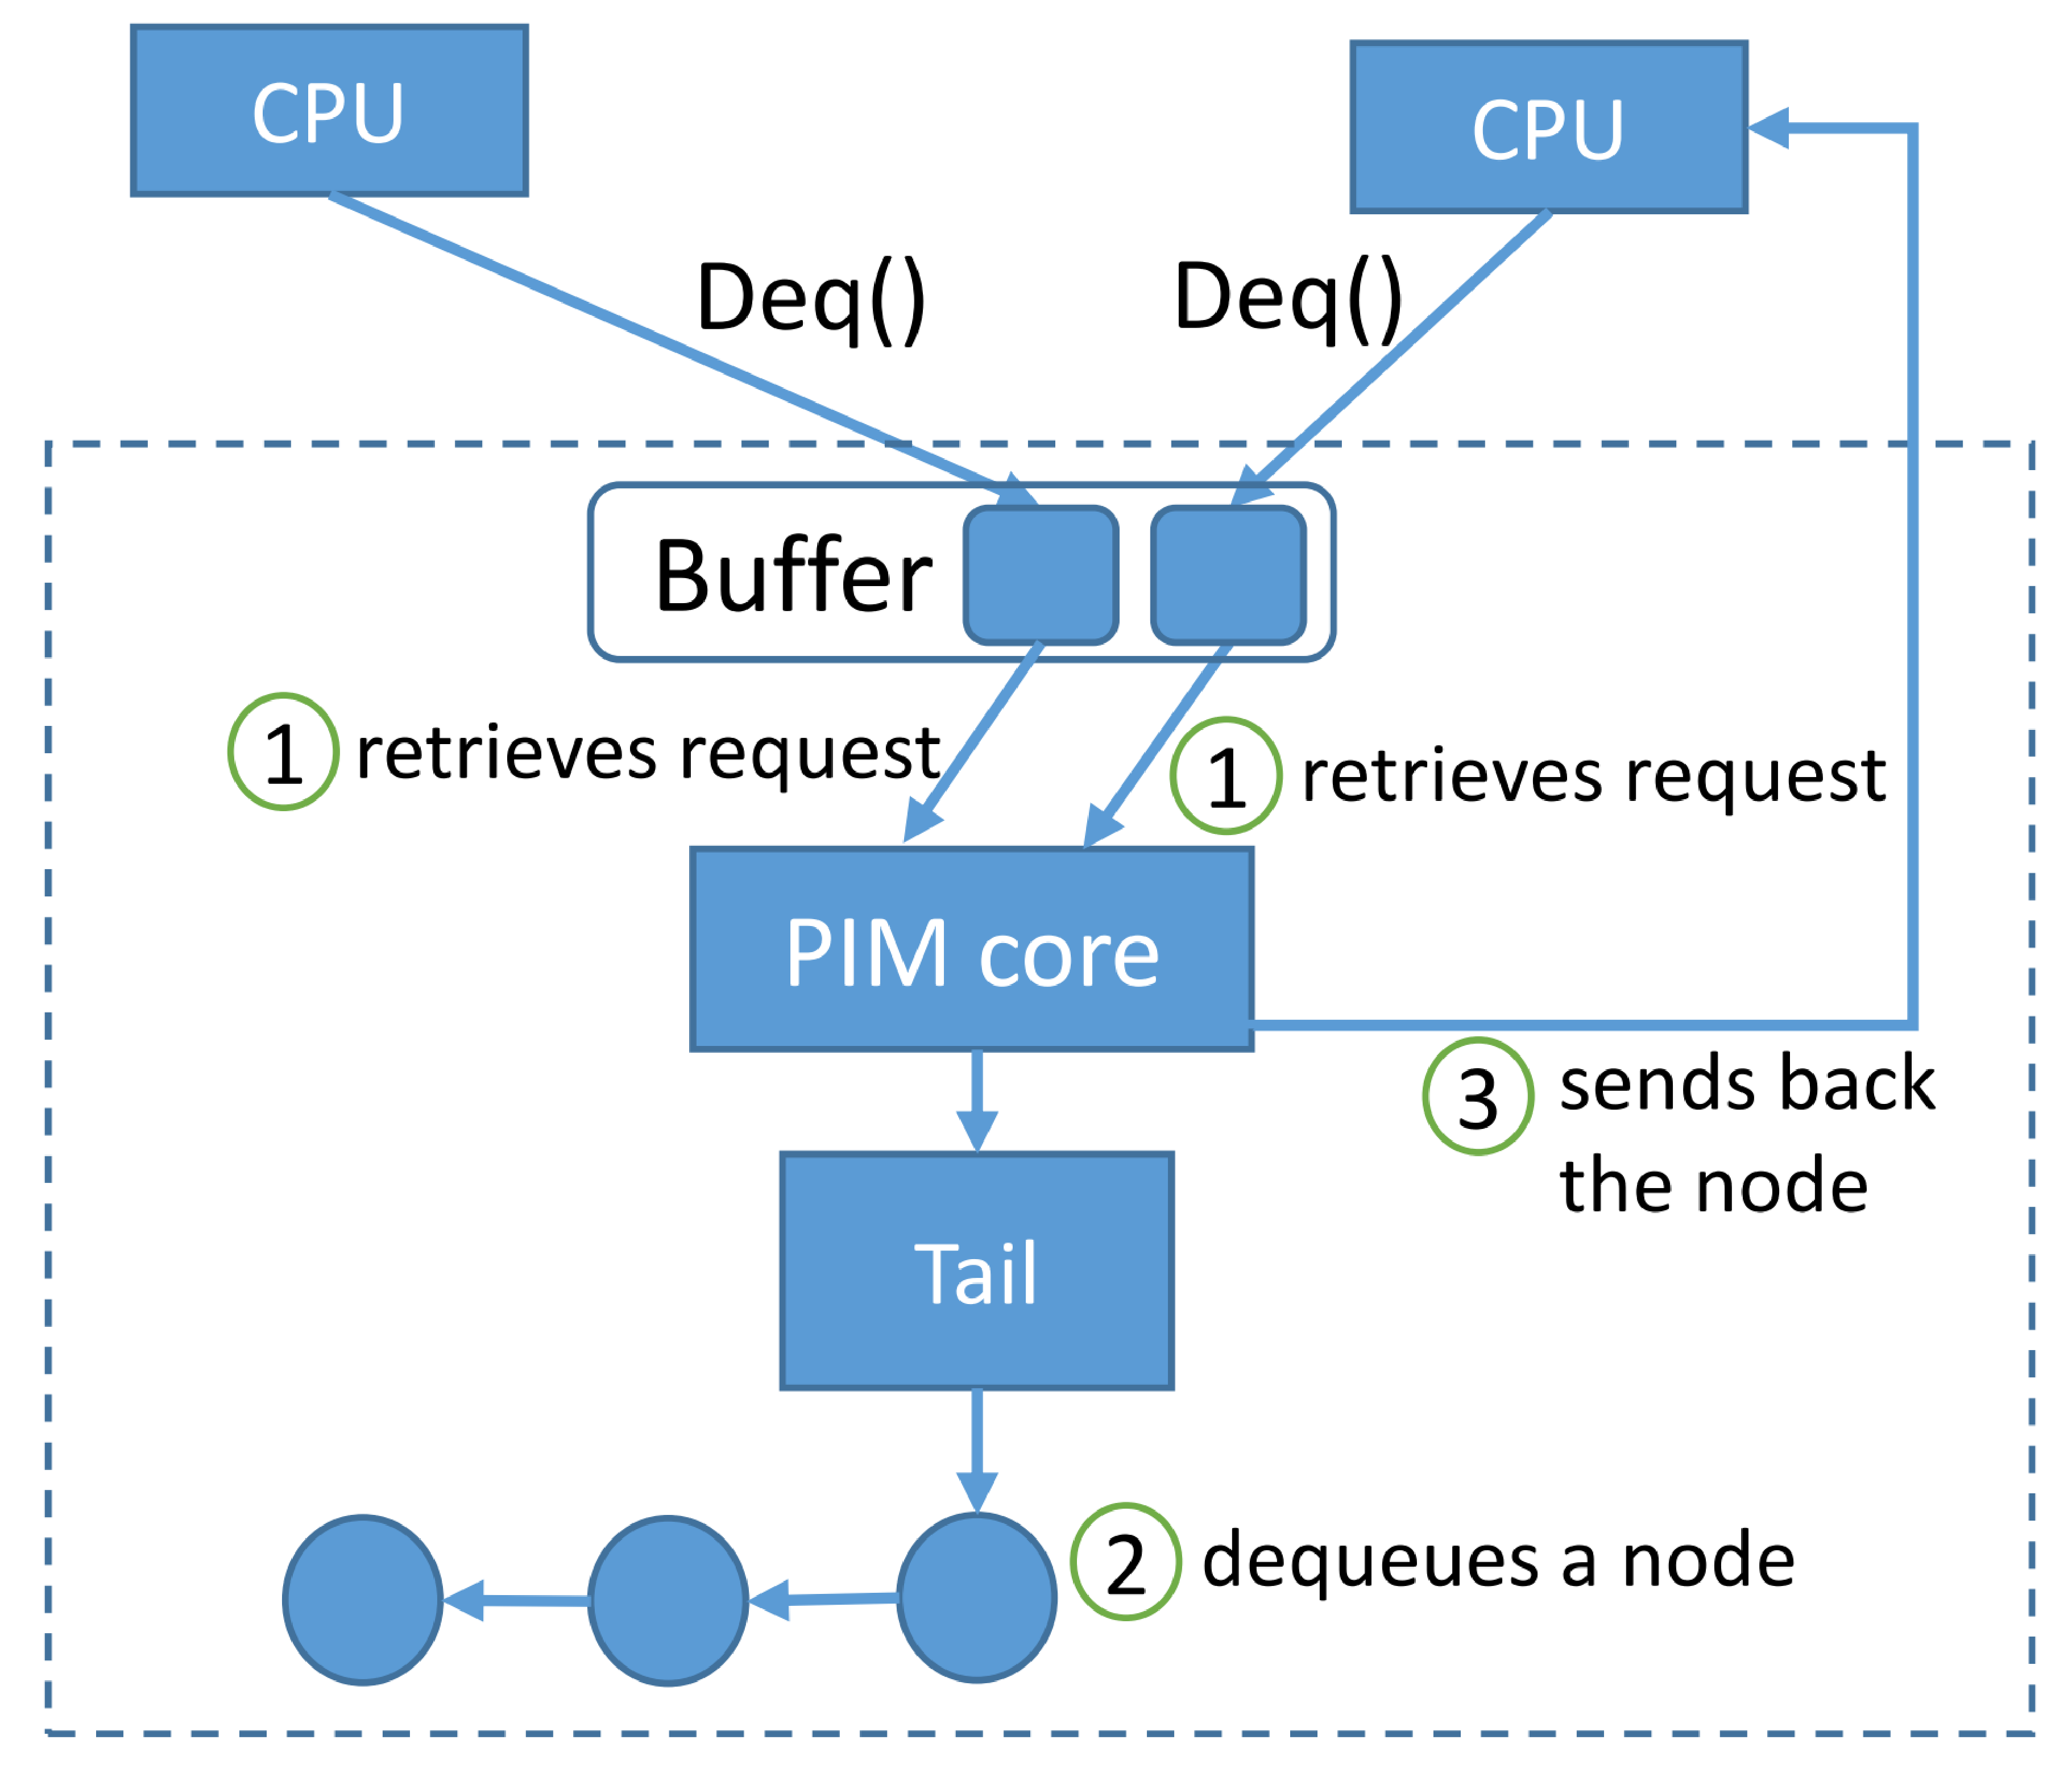
\includegraphics[width=.8\linewidth]{queue_pipeline.eps}}
\\
\subfigure[]{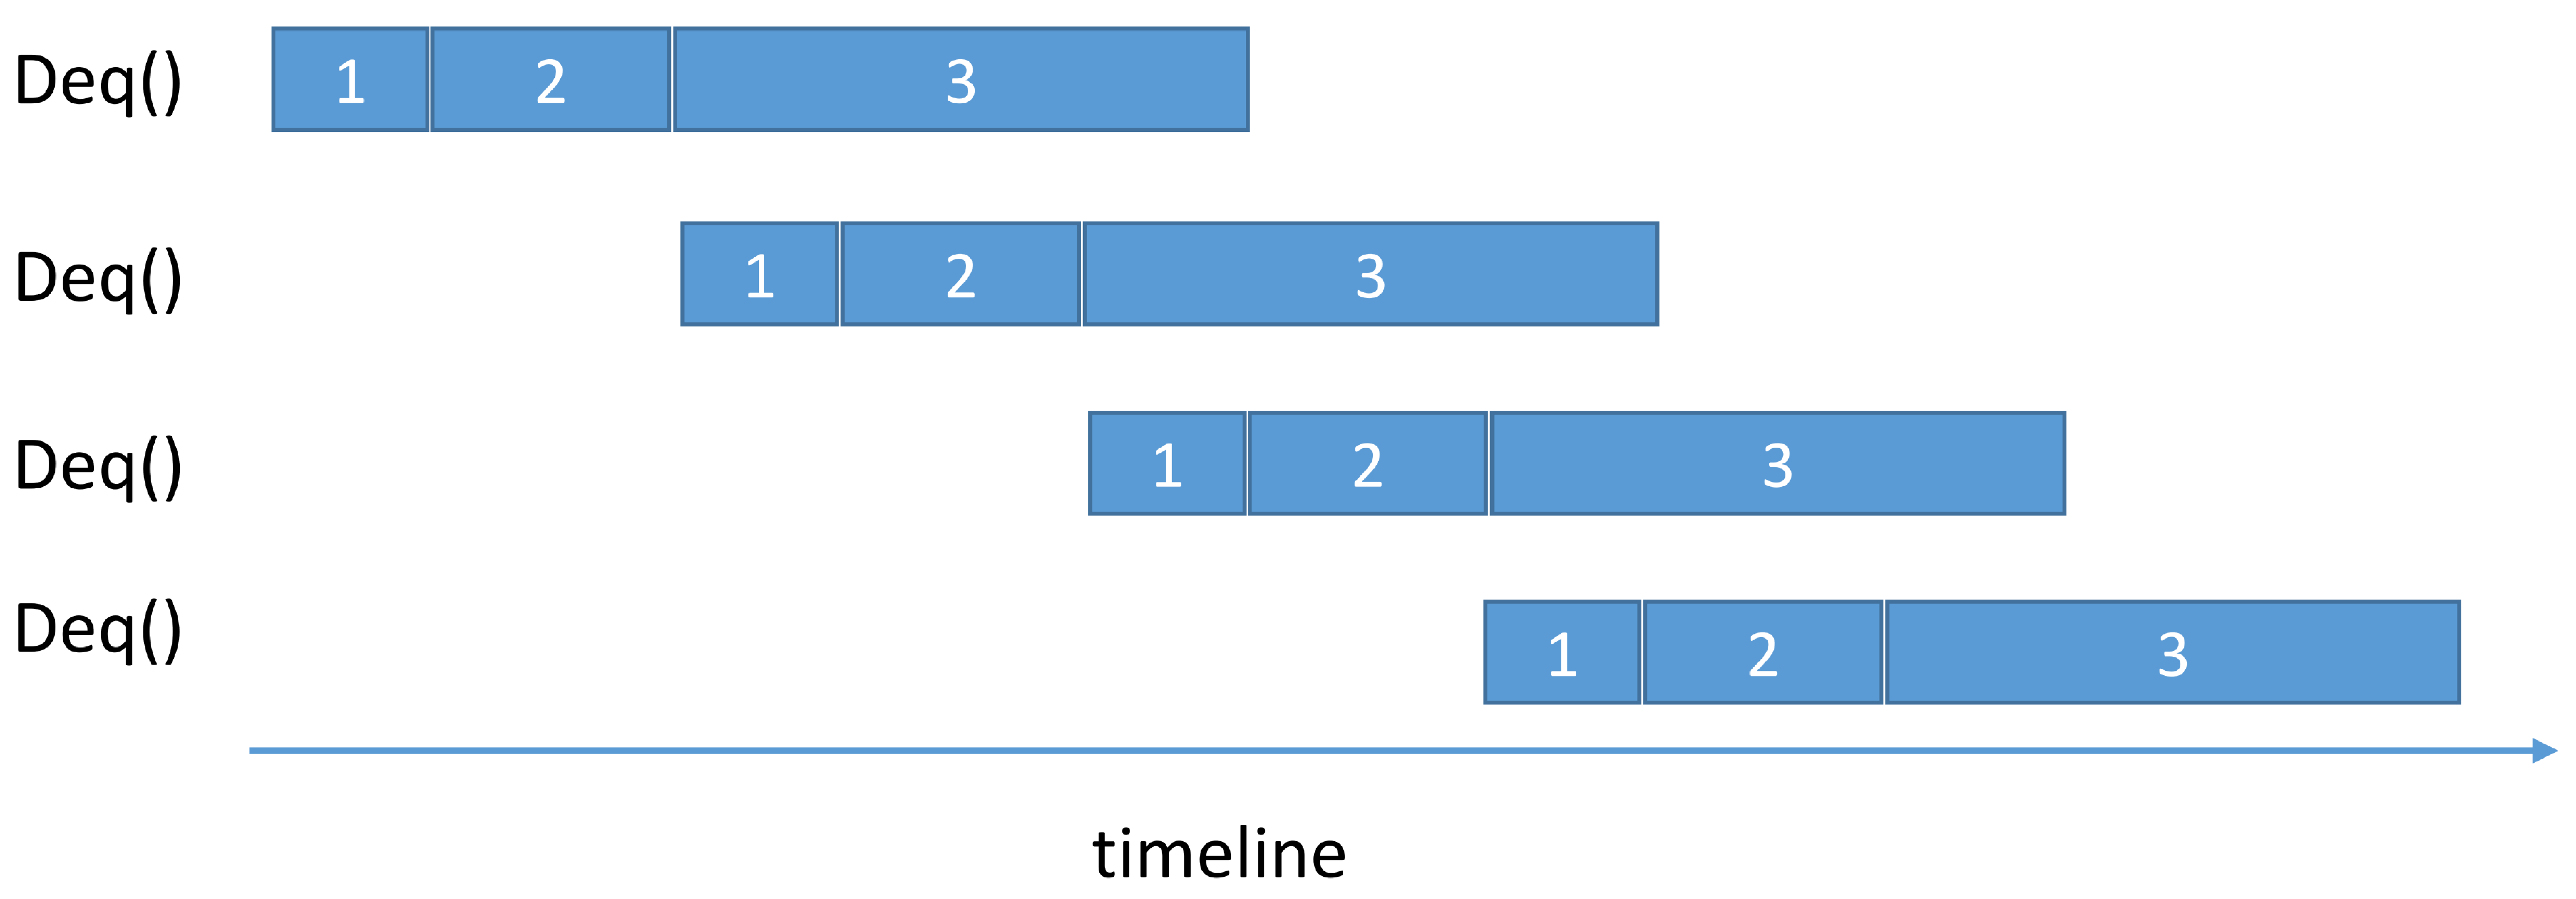
\includegraphics[width=1.0\linewidth]{queue_pipeline_timeline.eps}}

%$\hrulefill$
\caption{(a) illustrates the pipelining optimization, where a PIM core can start executing 
a new deq() (step 1 of deq() for the CPU on the left), without waiting for the dequeued node of 
the previous deq() to return to the CPU on the right (step 3). 
(b) shows the timeline of pipelining four deq() requests.}
\label{figure:queue_pipeline}
\end{figure}

The performance of our PIM-managed FIFO queue seems poor at first sight: although a PIM core can update 
the queue efficiently, it takes a lot of time for the PIM core to send results back to CPUs one by one. 
To improve its performance, the PIM core can \textit{pipeline} the executions of requests, 
as illustrated in Figure \ref{figure:queue_pipeline}(a). 
Suppose $p$ CPUs send $p$ dequeue requests concurrently to the PIM core, which takes time $\latmes$. 
The PIM core fist retrieves a request from its message buffer (step 1 in the figure), 
dequeues a node (step 2) for the request, and sends the node back to the CPU (step 3). 
After the PIM core sends off the message containing the node, it immediately retrieves the next 
request, without waiting for the message to arrive at its receiver. 
This way, the PIM core can pipeline requests by overlapping the latency of message transfer (step 3) 
and the latency of memory accesses and local computations (steps 1 and 2) in multiple requests 
(see Figure \ref{figure:queue_pipeline}(b)). 
During the execution of a dequeue, the PIM core only makes one memory access to read the node 
to be dequeued, and two L1 cache accesses to read and modify the tail node of the dequeue segment.  
It is easy to prove that the execution time of $p$ requests, including the time CPUs send 
their requests to the PIM core, is only $\latmes + p(\latpim + \epsilon) + \latmes$, where $\epsilon$ 
is the total latency of the PIM core making L1 cache accesses and sending off one message, 
which is negligible in our performance model. 
If each CPU makes another request immediately after it receives the result of its previous request, 
we can prove that the throughput of the PIM-managed FIFO queue is 
$${1 - 2\latmes \over \latpim + \epsilon} \approx {1 - 2\latmes \over \latpim} 
\approx {1 \over \latpim},$$
which is expected twice the throughput of the flat-combining queue and 
three times that of the F\&A queue, in our performance model 
assuming $\latato = 3\latllc = 3\latpim$. 

When the PIM-managed FIFO queue is short, it may contain only one segment 
which deals with both enqueue and dequeue requests. 
In this case, its throughput is only half of the throughput shown above, 
but it is still at least as good as the throughput of the other two algorithms. 

We have preliminary experiments for the flat-combining queue and the F\&A-based queue. 
To be consistent with our analysis above, we have modified the two algorithms in order to 
measure the performance of the parts we focused in our analysis.  
More specifically, in the flat-combining queue, the combiner does not make 
real enqueue or dequeue operations for requests. 
Instead, after retrieving a request from the publication list, 
the combiner simply waits time $t_1$ and then writes a fake result back, 
where $t_1$ is the average execution time of an enqueue in the original algorithm. 
This way, we can easily use Linux perf to count the last-level cache accesses incurred 
on the publication list, in which we are interested, 
while simulating the rest of the algorithm we omit. 
In the F\&A-based queue, each thread only makes a F\&A operation on one of the two shared objects 
to compete for a slot of the queue, and the rest of the algorithm, 
which does the real enqueue and dequeue operations, is omitted. 
Again, to simulate the latency of the operations omitted, each thread stays idle for time $t_2$ 
after the F\&A operation, where $t_2$ is the average execution time of those operations 
in the original algorithm.

The experiments were run on a machine with 14 cores, each having two hyperthreads. 
To evaluate the algorithms with and without hyperthreading, we chose two settings for the experiments: 
1) (without hyperthreading) for $1 \le n \le 14$, 
each of the $n$ threads was pinned to a hyperthread of a different core, and
2) (with hyperthreading) for $1 \le n \le 28$ and any $1\le i \le n/2$, 
the $i$th pair of threads were pinned to the two hyperthreads of the $i$th core respectively. 
The results of our experiments are presented in Figure \ref{figure:FC_FandA_queues}. 
In each experiment, each thread made $10^7$ requests and 
we counted the average number of last-level cache accesses a request incurred. 

In the the Flat-combining queue without hyperthreading (Figure \ref{figure:FC_FandA_queues}(a)), 
each request incurred on average roughly 4.8-4.9 last-level cache accesses. 
Note that a thread submitting a request usually makes at most 3 last-level cache accesses---one 
when it writes the request into the publication list, one when it tries to acquires the lock, 
one when it reads the result returned by the combiner. 
(A thread may retry to acquire the lock, incurring more last-level cache accesses, 
if its request was missed by the previous combiner. 
However, this situation happened rarely in our experiments and therefore its impact can be ignored.) 
Thus, we can conclude that the combiner incurred at least 1.8-1.9 last-level cache accesses 
on average per request, and this result is very close to our expectation (i.e., $2\latllc$ per request). 
With hyperthreading(Figure \ref{figure:FC_FandA_queues}(b)), 
each request incurred 4.0-4.5 last-level cache accesses when we had more than 10 threads, 
and therefore the combiner incurred at least 1.0-1.5 last-level cache accesses per request. 
Although this improves the performance by 90\%-20\%, our PIM-managed queue is still better in theory, 
given that the performance of our algorithm is expected twice the performance of 
the Flat-combining queue without hyperthreading in our performance model. 

In the F\&A-based queue without hyperthreading (Figure \ref{figure:FC_FandA_queues}(c)), 
each request incurred almost one last-level cache access, which is a F\&A operation, 
meeting our expectation (i.e., $\latato$ per request) in earlier analysis. 
With hyperthreading (Figure \ref{figure:FC_FandA_queues}(d)), each request made roughly 
0.55-0.8 last-level cache access by F\&A. 
Even if we think F\&A on L1 and L2 caches by F\&A is cheap and negligible, 
the performance of the algorithm improves only by 82\%-25\%, which is still worse than 
the PIM-managed queue's expected performance. 


% \begin{figure}[ht!]
% %$\hrulefill$
% %\\
% %\\
% \centering
% \subfigure[]{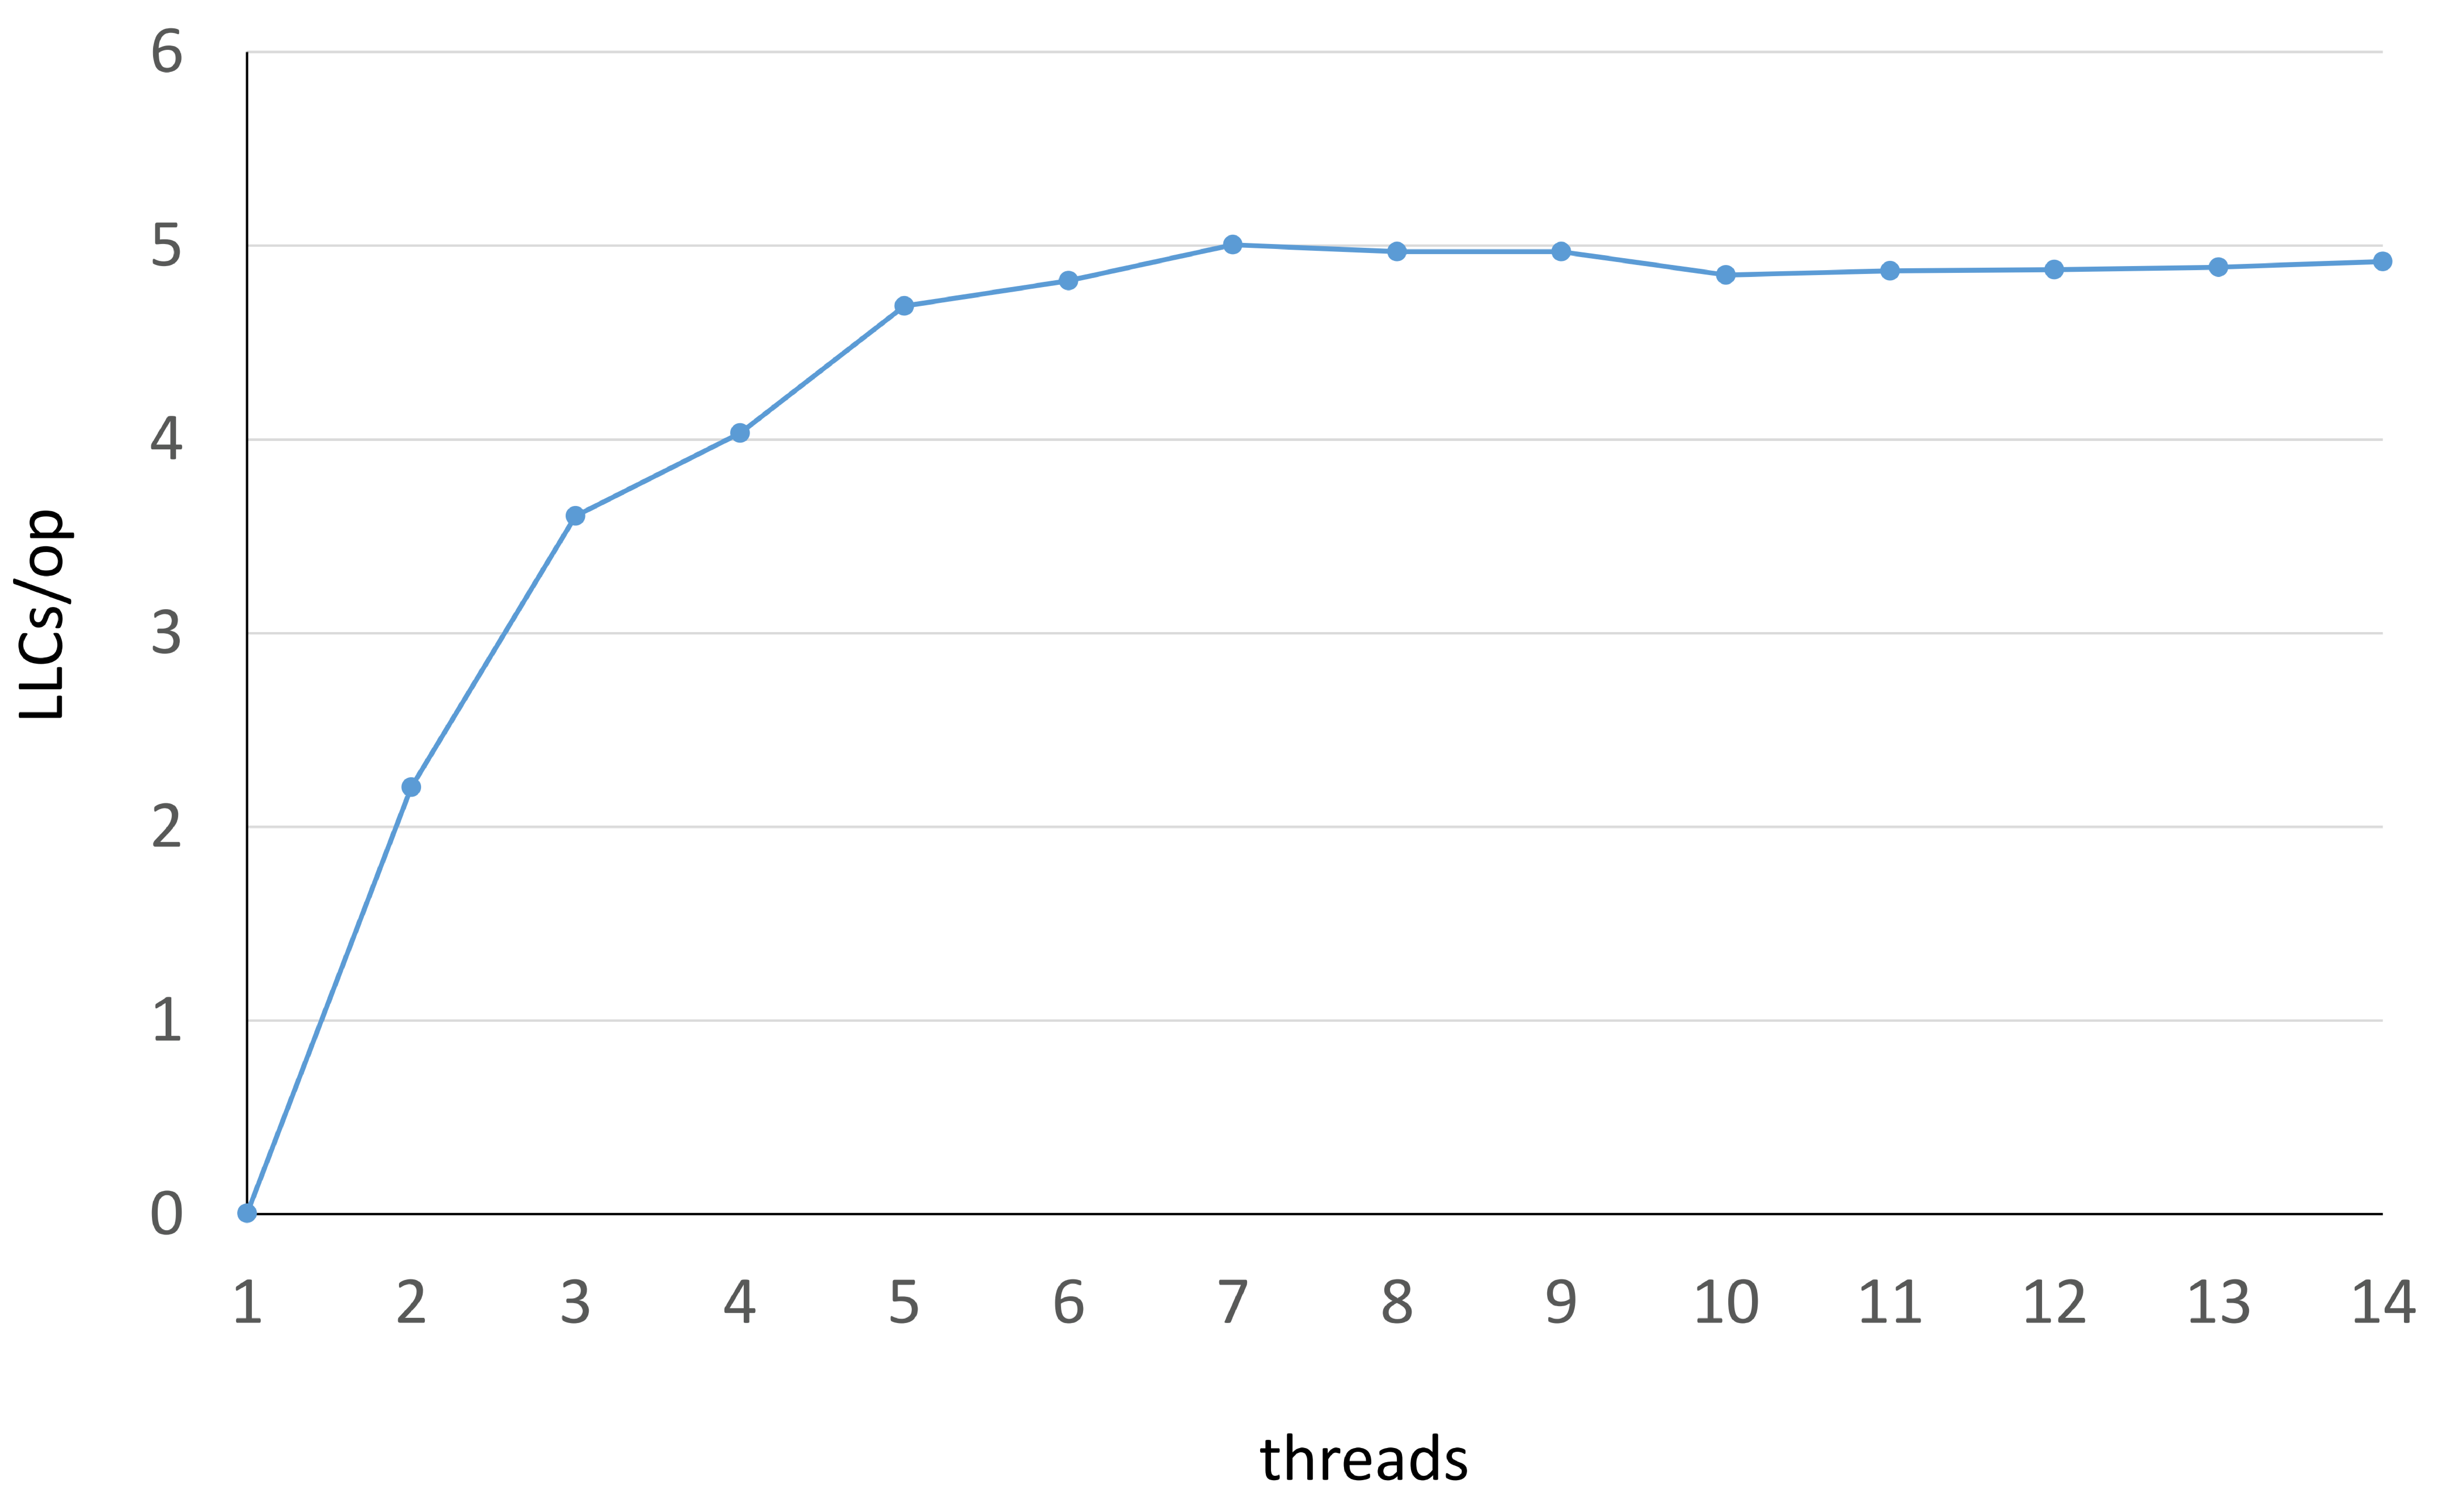
\includegraphics[width=.9\linewidth]{queue_FC.eps}}
% %\subfigure[]{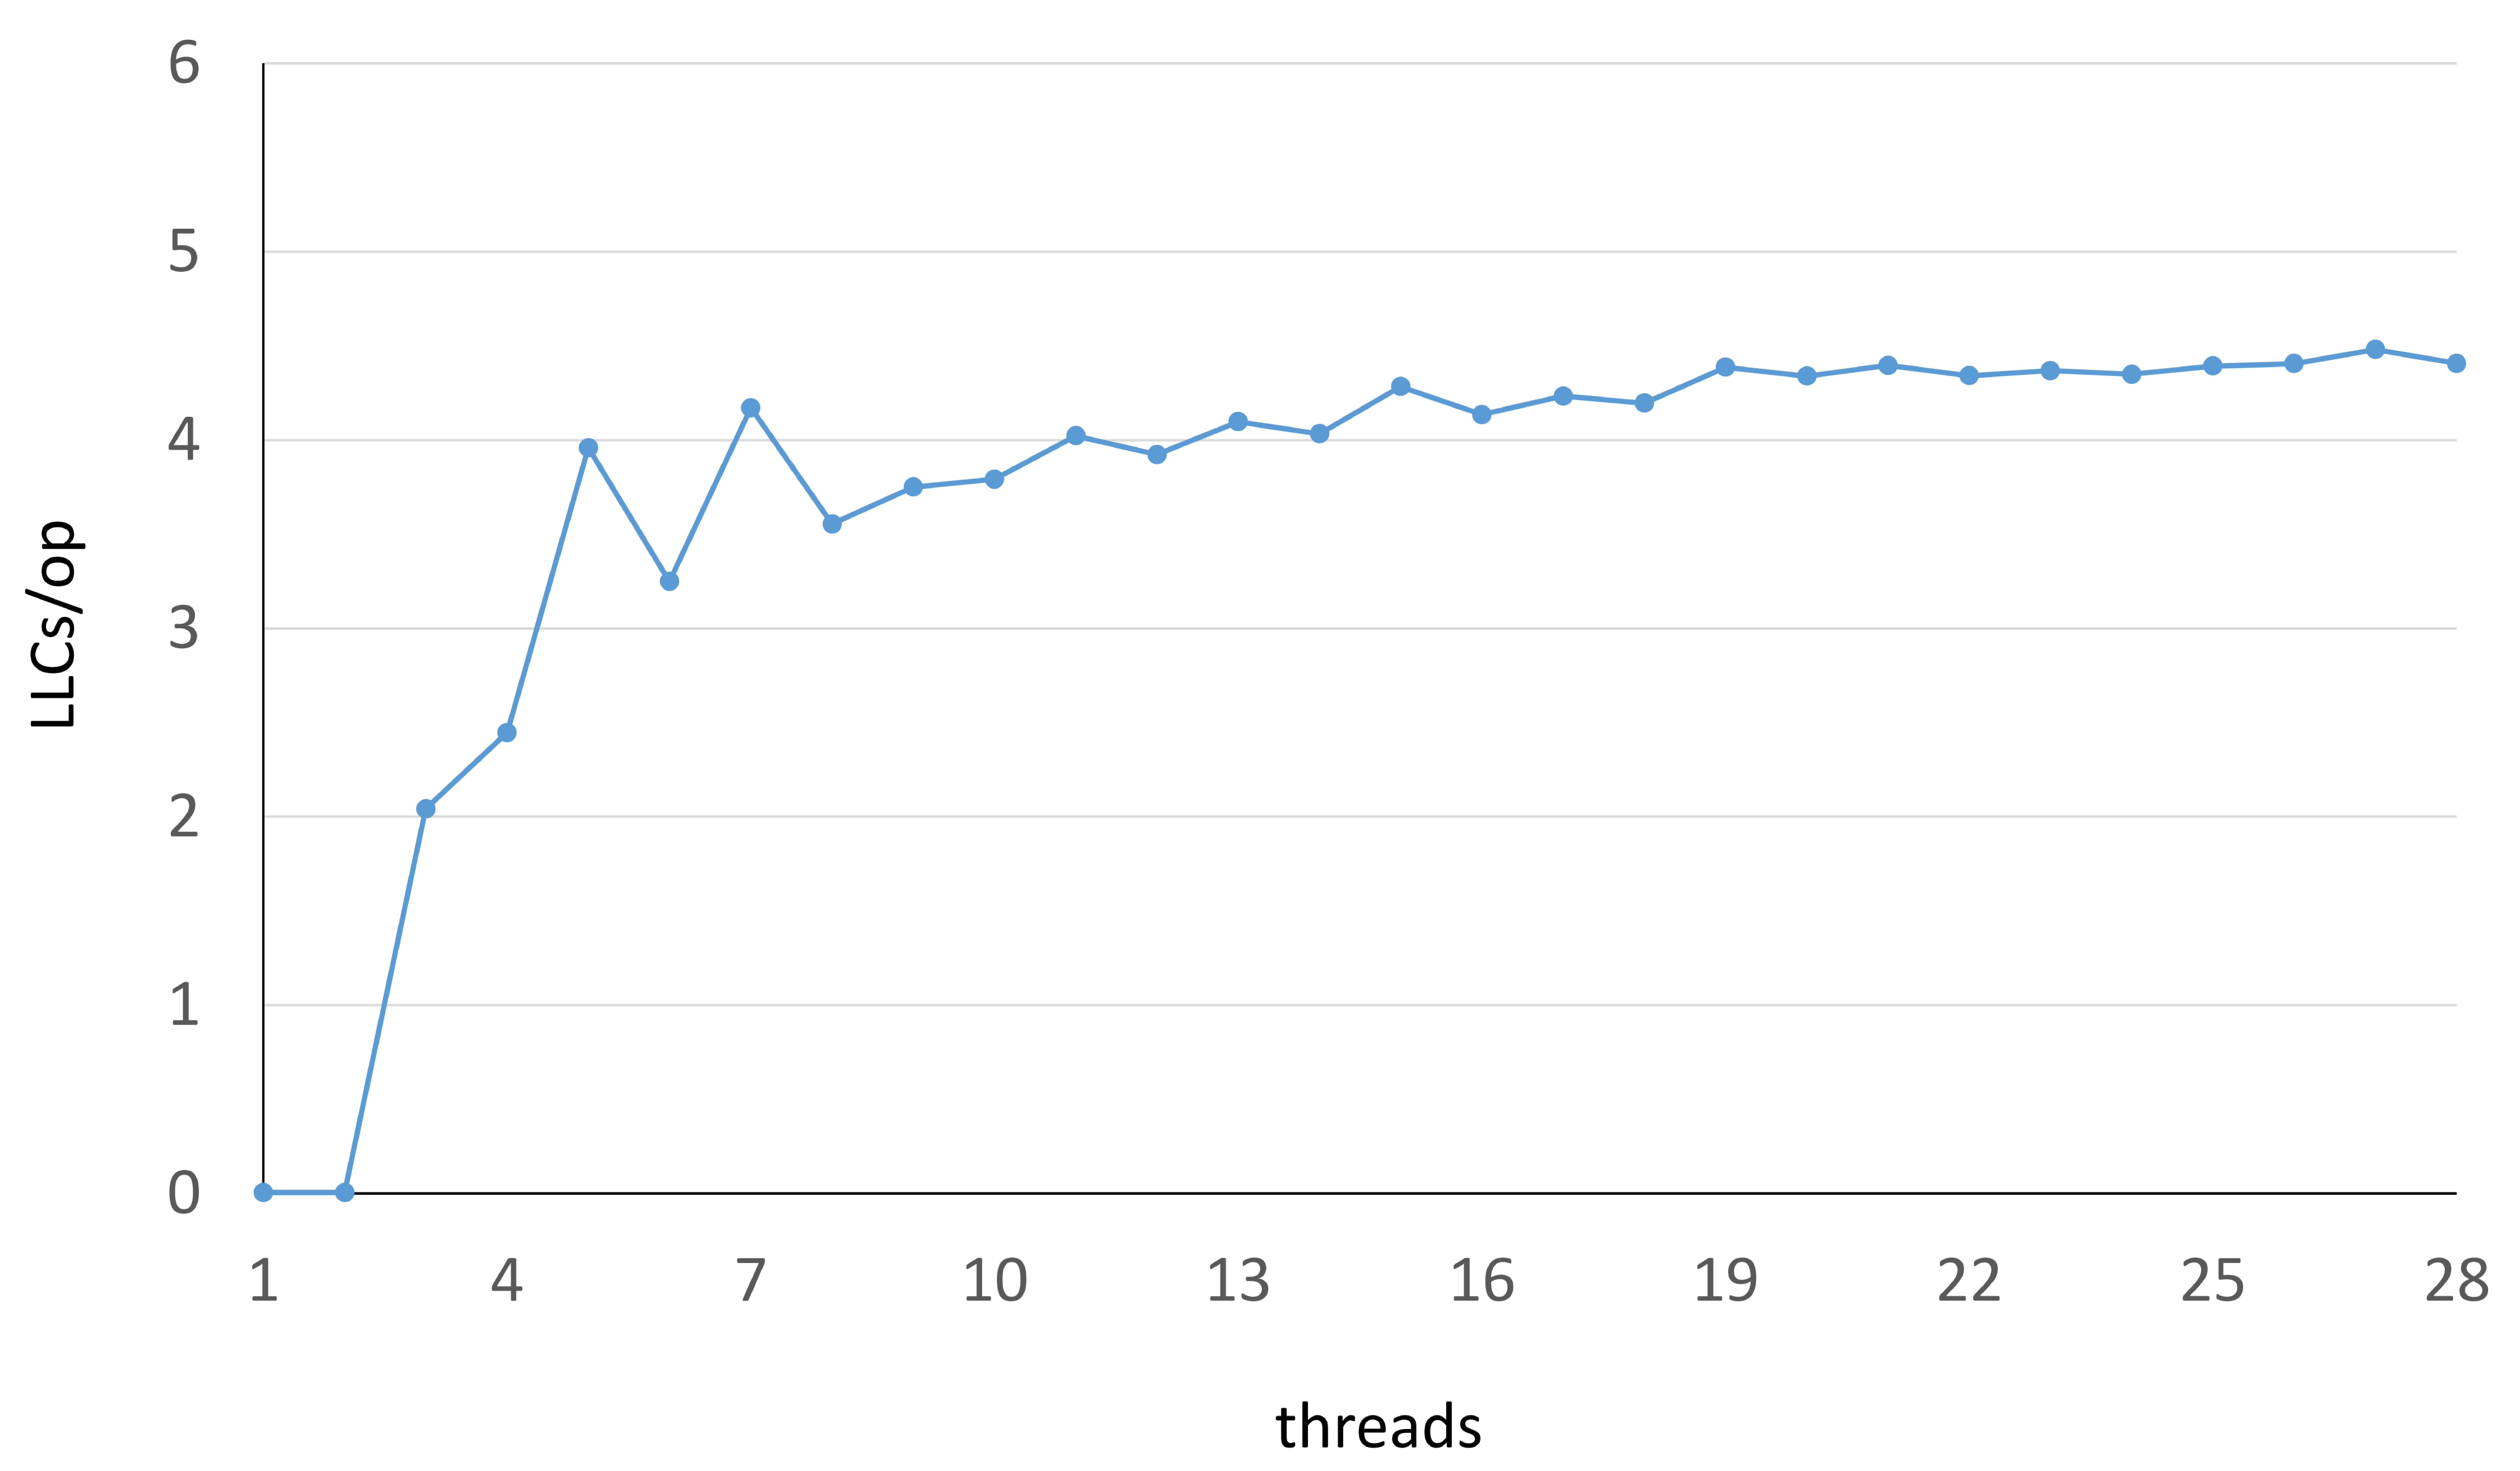
\includegraphics[width=.45\linewidth]{queue_FC_hyperthreads.eps}}
% \subfigure[]{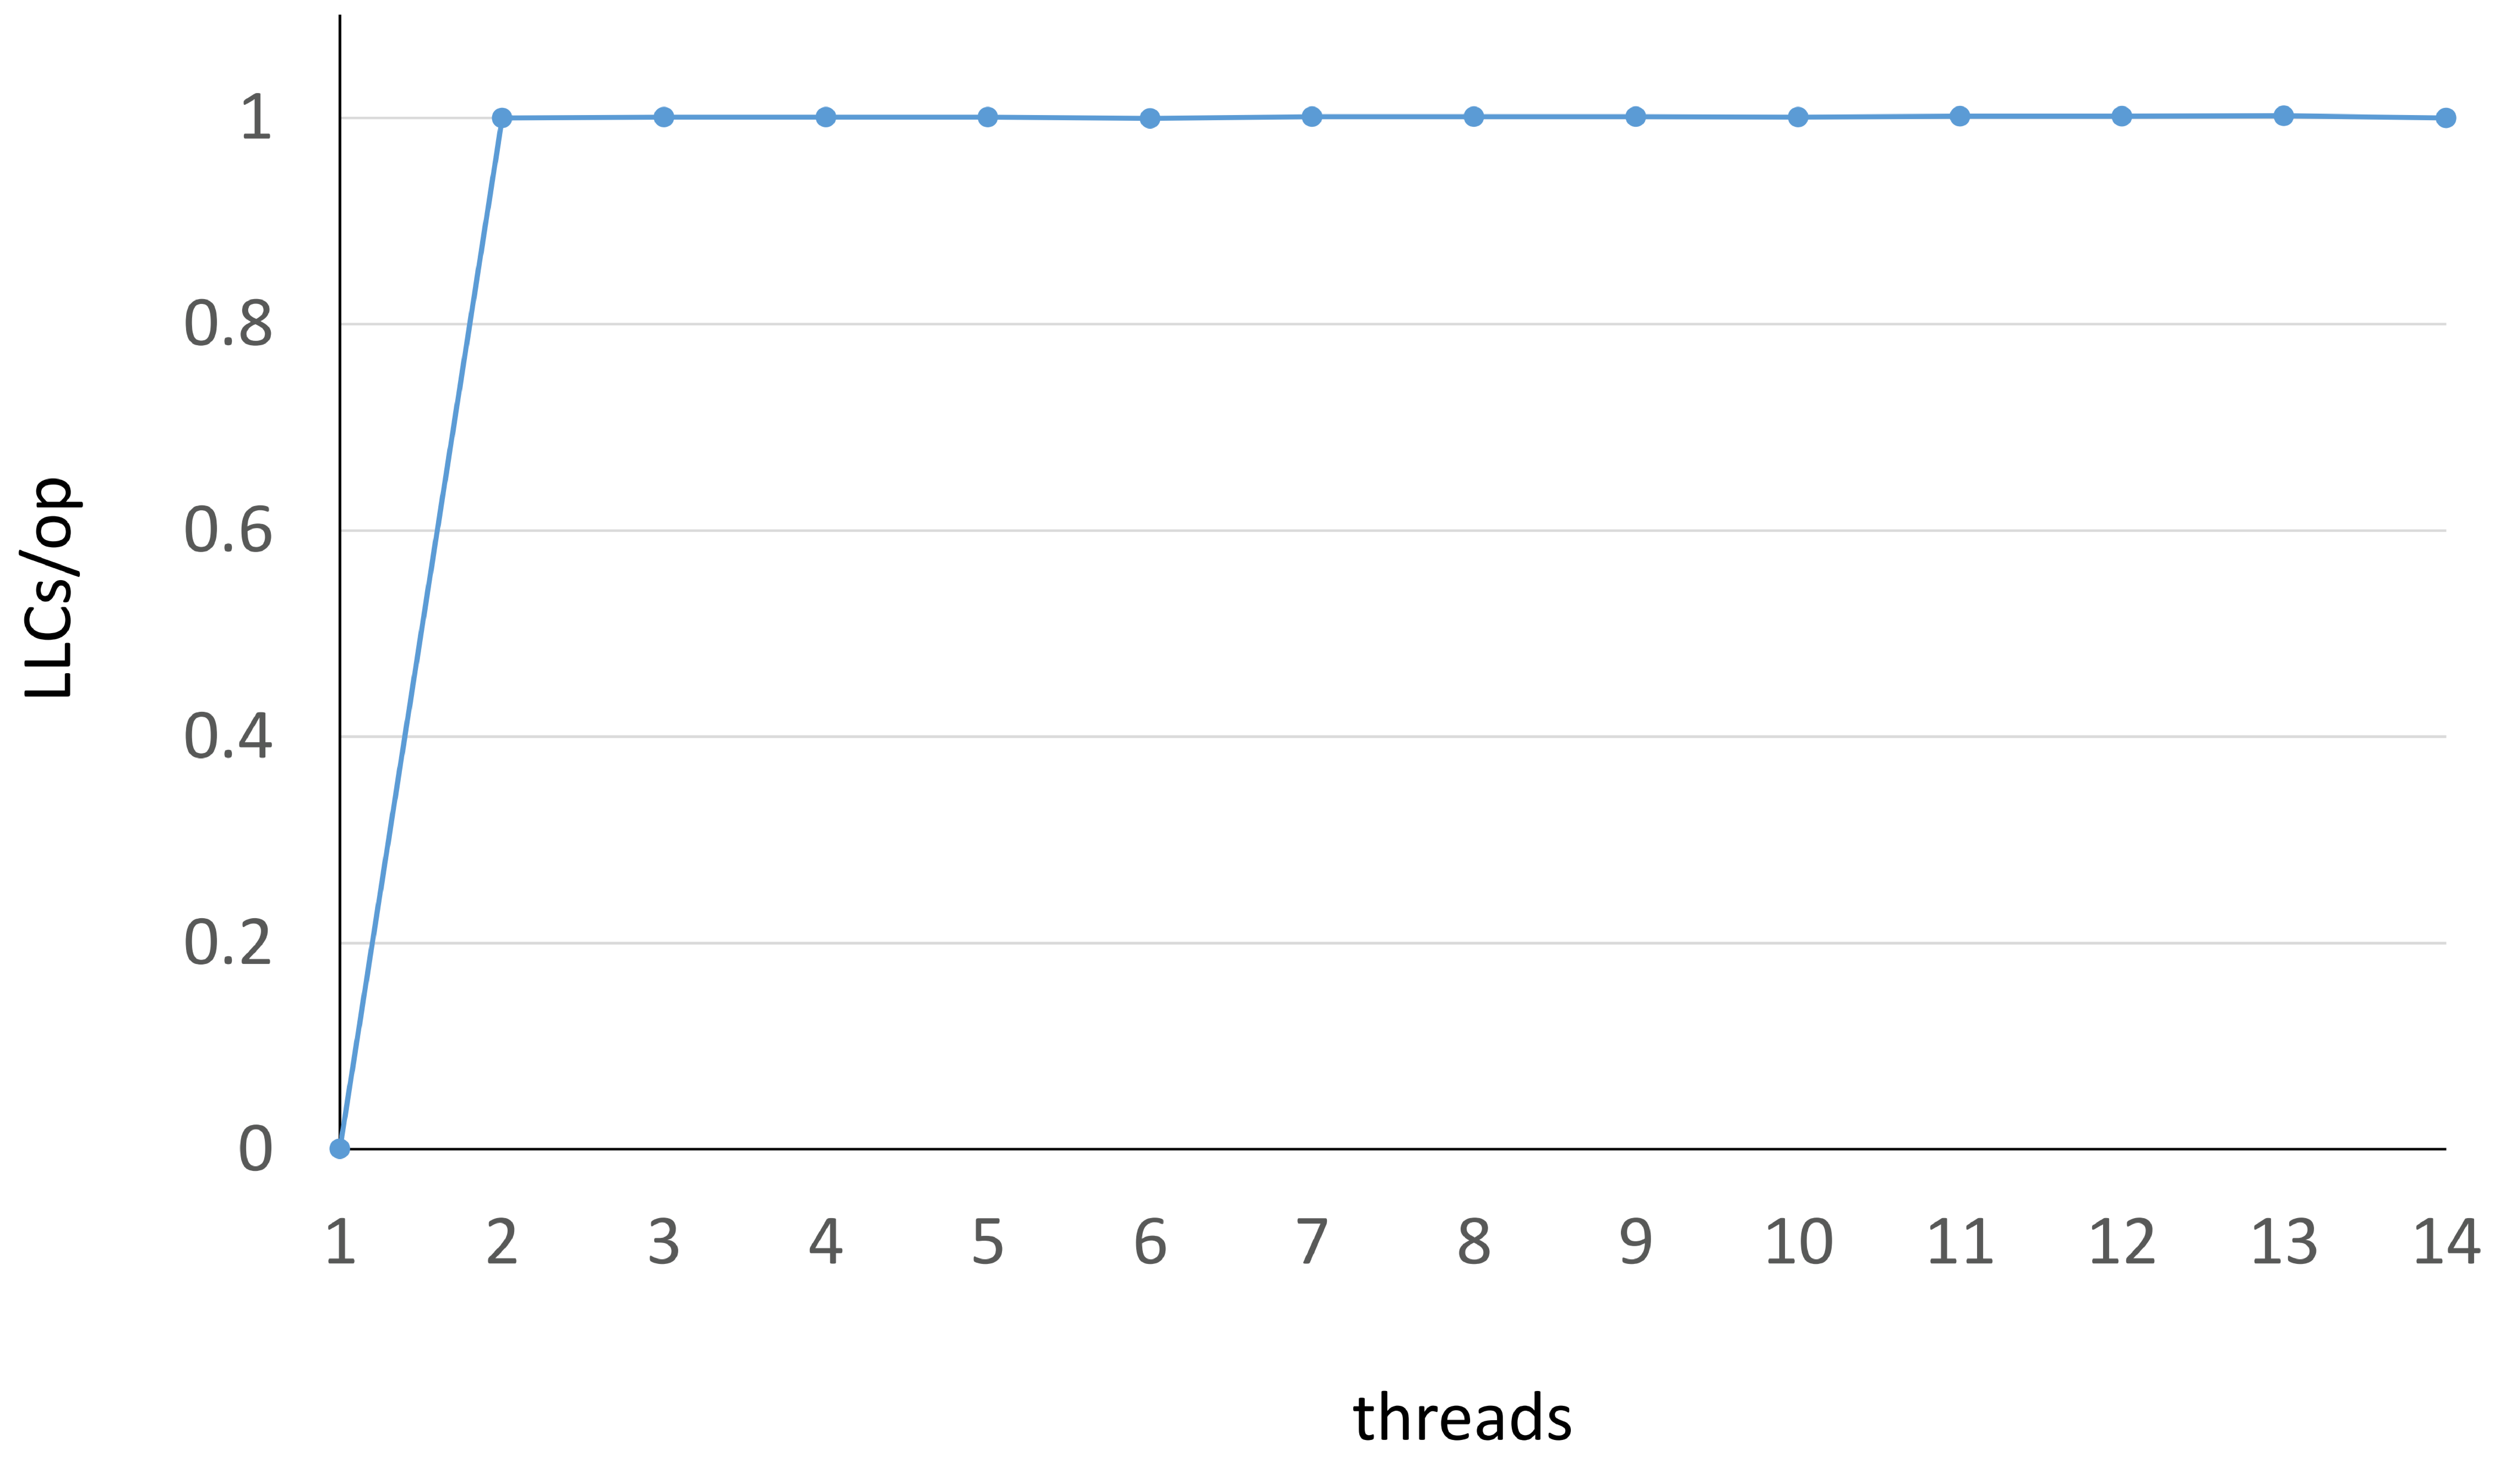
\includegraphics[width=.9\linewidth]{queue_FandA.eps}}
% %\subfigure[]{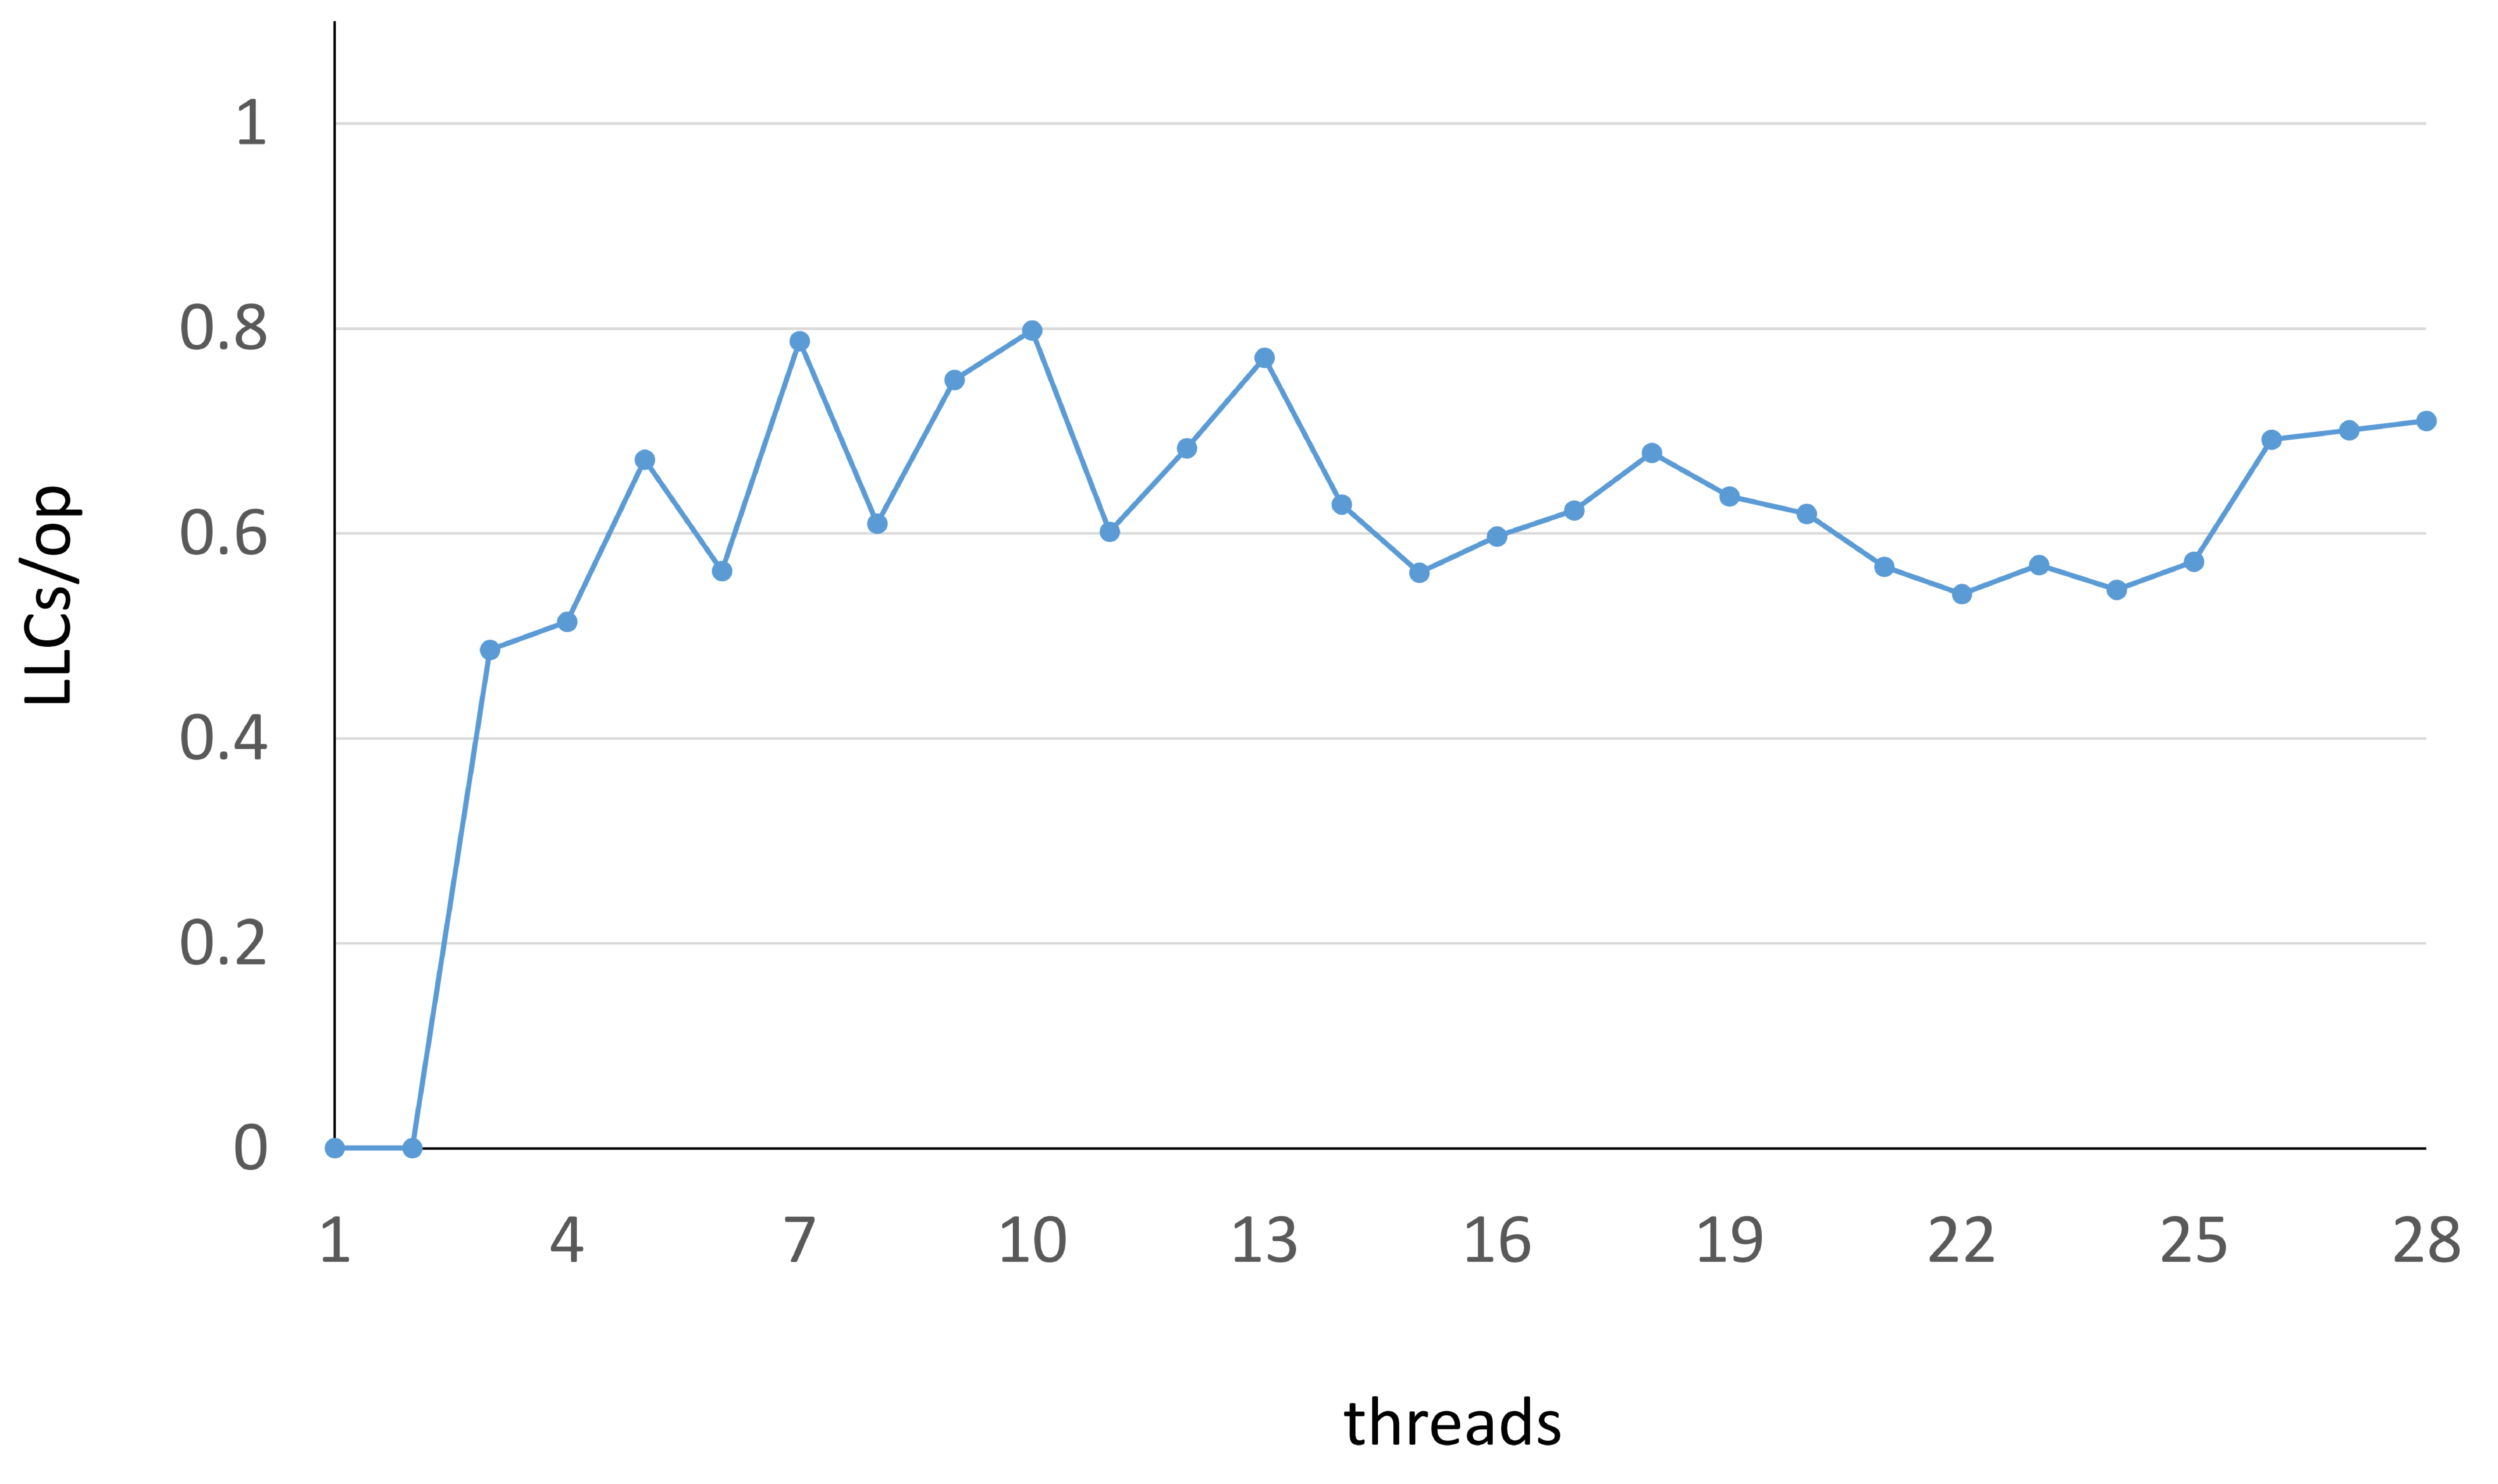
\includegraphics[width=.45\linewidth]{queue_FandA_hyperthreads.eps}}
% 
% %$\hrulefill$
% \caption{(a) Flat-combining queue. (b) F\&A-based queue without hyperthreading.}
% \label{figure:FC_FandA_queues}
% \end{figure}